\documentclass[conference]{IEEEtran}
\IEEEoverridecommandlockouts
% The preceding line is only needed to identify funding in the first footnote. If that is unneeded, please comment it out.
\usepackage{cite}
\usepackage[portuges,brazil,english]{babel}
\usepackage[utf8]{inputenc}
\usepackage{hyperref}
\usepackage{amsmath,amssymb,amsfonts}
\usepackage{amsmath}
\usepackage{algorithm}
\usepackage{algorithmic}
\usepackage{graphicx}
\usepackage{textcomp}
\DeclareUnicodeCharacter{00A0}{ }
\def\BibTeX{{\rm B\kern-.05em{\sc i\kern-.025em b}\kern-.08em
    T\kern-.1667em\lower.7ex\hbox{E}\kern-.125emX}}
\begin{document}

\title{Clusterização de emails}

\author{\IEEEauthorblockN{André Almeida}
\IEEEauthorblockA{
RA: 164047 \\
\texttt{fda.andre@gmail.com}}
\and
\IEEEauthorblockN{Igor Torrente}
\IEEEauthorblockA{
RA: 169820 \\
\texttt{igortorrente@hotmail.com}}}

\maketitle



\section{Resumo}

Nesse trabalho, estudamos técnicas de aprendizado de máquina e reconhecimento de padrões para obter um modelo de \textit{clusterização} automática de emails em assuntos a partir do texto do email.

\section{Introdução}

\subsection{Classificador automático de emails}

Classificar emails automaticamente é um problema explorado por empresas provedoras de serviço de email. Uma classificação importante para manter a qualidade do serviço é a classificação binária \textit{spam} (mensagens indesejadas com propaganda ou com golpes cibernéticos) / não \textit{spam}\cite{b1}, de forma a deixar a caixa de entrada dos usuários livres de conteúdo indesejado. Uma outra funcionalidade que a classificação automatizada pode trazer é separar os assuntos dos usuários entre atualizações, redes sociais, fóruns, etc., como faz o serviço de email do Google, o Gmail\cite{b2}.

\subsection{Clustering}
Algoritmos de \textit{clusterização} dividem dados em grupos (clusters) baseados apenas nas informações providenciadas pelos dados. O objetivo é conseguir agrupar em um mesmo grupo dados similares/relacionados e dados que sejam diferentes estarem em grupos diferentes. Quanto mais parecidos os dados de um grupo forem, e quanto maior a diferença entre grupos distintos, melhor será a clusterização desses dados. Em alguns algoritmos, o número de clusters é definido pelo usuário (e.g. \textit{K-means}) e em outros o algoritmo tenta encontrar o número ideal de clusters (e.g. \textit{DBSCAN}) \cite{b3}. Nesse estudo, exploramos o primeiro tipo, especificamente o \textit{K-means}. Esse tipo de técnica é considerada de aprendizagem não-supervisionada. Ao contrário das técnicas de aprendizado supervisionadas, os dados não possuem previamente nenhum tipo de classe ou rótulo.

\subsubsection{K-means}
Esse algoritmo de clusterização é o mais antigo e mais usado. A ideia dele é encontrar \textit{K} centroides (onde \textit{K} é um parâmetro definido pelo usuário), onde um centroide é a média de um grupo de pontos. As primeiras localizações dos centroides podem ser aleatórias. Cada ponto é então atribuído ao centroide mais próximo, e um grupo de pontos de um mesmo centroide formam um cluster. O centroide é atualizado baseado na média dos pontos do seu cluster. O algoritmo continua assim até que não ocorra mais atualizações nos pontos dos clusters\cite{b3}. Uma simplificação do algoritmo pode ser definida como:
\linebreak

\begin{algorithm}
\caption{K-Means}
\begin{algorithmic}[1]
\STATE Selecione \textit{K} pontos como os centroides iniciais;
\REPEAT
	\STATE Forme os \textit{K} clusters atribuido cada ponto ao seu centroide mais próximo;
	\STATE Reposicione os centroides de cada cluester;
\UNTIL Centroides não mudem.
\end{algorithmic}
\end{algorithm}

 
\subsection{Base de dados}
A base de dados consiste de em um conjunto de e-mails do anos 90 que pertencem a grupos de noticias, cada e-mail possui um newsgroup a que ele pertence, um assunto, datas, o corpo do e-mail e outros metadados relacionados. \cite{b4}

\subsection{Tecnologias empregadas}
Utilizamos a biblioteca \textit{sklearn}\cite{b5} do \textit{Python} para as chamadas de pre-processamento de dados e clusterização. O \textit{Jupyter} foi escolhido como ambiente de desenvolvimento.

\subsection{Infraestrutura computacional}
Os recurso computacionais foram:

\begin{itemize}
\item Computador com um processador Intel Core i7-3537U (2.00GHz × 4) e com 7,7 GiB disponíveis de memória RAM com Arch Linux;

\item Máquina virtual com 4 núcleos virtuais do processor IBM Power8, com 16GB de RAM e  Ubuntu 17.04;

\item Computador com core i5 4440, 8 GB de Ram e Windows 10.

\end{itemize}

\section{Tratamento de dados}

Para conseguir extrair as informações necessárias dos textos, não necessitamos do texto integral do email. O cabeçalho contendo os metadados do email provavelmente não diz muito sobre o conteúdo do corpo do texto. A base de dados proposta para o experimento (\textit{data.csv}) contêm cerca 2.209 palavras, do total de 2 milhões de palavras únicas encontradas nos arquivos. Essa base de dados é do tipo \textit{bag-of-words}, com a frequência de cada termo dividido pela quantidade de emails em que ela aparece.\\
Também foram exploradas outras maneiras de reduzir o conteúdo dos arquivos. Utilizamos redução de dimensionalidade com PCA no \texttt{data.csv} e criamos novos conjuntos de dados usando \textit{stemming} e \textit{stopwords} nos emails brutos.

\subsection{Bag-of-words}
O \textit{bag-of-words} é um modelo de representação textual comumente usada para classificação de texto. Ele reserva uma posição do vetor a cada palavra utilizada no texto ou conjunto de textos, existem três formas comuns de se utilizar a \textit{bag-of-words}\cite{b10}
\begin{enumerate}
\item Uma que se utiliza a posição reservada para contar a quantidade de vezes que a palavra foi usada no texto ou conjunto de textos;
\item Cada posição do vetor guarda a frequência que o termo aparece divida pelo total de palavras do texto, esse modelo é chamado de bag of words TF (\textit{Term frequecy});
\item Por fim cada posição guarda a relevância estatística do termo em relação a sua frequência no conjunto de textos. A relevância é calculada como o TF dividido pela quantidade de textos que aquela palavra aparece. Esse mode é chamado de bag of words TF-IDF (\textit{requency-inverse document frequency}).
\end{enumerate}

\subsection{Stemming}
A  técnica de \textit{stemming} reduz a palavra para sua raíz morfológica, similar à recuperar o radical de uma palavra. Um exemplo seria aplicar \textit{stemming} em "correr", "correndo" e "corria", onde as três palavras se tornariam "corr". Isso é útil tanto para maximizar o significado das palavras (conjugações diferentes do mesmo verbo contem um significado muito próximo) quanto reduzir o número de dados. Os \textit{stemmers} utilizados foram: \textit{Snowball}\cite{b6}, \textit{Wordnet}\cite{b7}, \textit{Porter}\cite{b8} e \textit{Lancaster}\cite{b9}, todos importados da biblioteca de processamento de linguagem natural do Python, NLTK\cite{b14}. Os textos que passaram por stemming também tiveram todas suas palavras convertidas para a forma minúscula.

\subsection{Stopwords}
\textit{Stopwords} são palavras muito comuns e sem muita relevância para o significado do texto, como "nós", "eu", "aquilo", "entre", "porque", etc. Removendo elas, diminuímos uma boa parte do volume de dados, já que as palavras mais comuns costumam ser \textit{stopwords}.

\subsection{Exemplos de tratamentos}
Aqui comparamos as 5 primeiras palavras mais populares entre alguns desses pré processamentos:

\begin{center}

    \begin{tabular}{ l }
    \textbf{Com \textit{stopwords}:} the, to, of, a, and, is.  \\
    \textbf{Sem \textit{stopwords}:} would, one, writes, dont, like.  \\
    \textbf{Após \textit{Lancaster}:} us, would, on, writes, artic. \\ 
    \end{tabular}
\newline

\end{center}

\section{Soluções propostas}
Nessa seção e nas próximas, as métricas para validar a eficiência do modelo são:
\begin{itemize}

\item \textit{\textbf{Score}}: O \textit{score} do \texttt{sklearn} para o K-Means é calculado por:
\begin{center}
 $(-1) \sum\limits_ {p  \thinspace \epsilon \thinspace Cluster} (centroid - p)^2 $
\end{center} 
Ele é usado para medir a distancia dos do centroide ao seu cluster identificando o cotovelo (\textit{elbow}) no gráfico de número de clusters pelo score \cite{b11}.

\item \textit{\textbf{Calinsk}}: O índice de Calinsk é dada pela razão entre as dispersões médias dos cluster pela dispersão do próprio cluster \cite{b12}.

\item \textit{\textbf{Silhouette}}: Para cada objeto \textit{i} obtêm-se o valor s(\textit{i})

\begin{center}
$s(\mathit{i}) = \frac{b \mathit{i} - a \mathit{i}}{max(a \mathit{i}, b\mathit{i})}$
\end{center}

onde:
  a\textsubscript{i} é a dissimilaridade média do objeto \textit{i} em relação a todos os outros objetos do seu cluster.
  b\textsubscript{i} é a dissimilaridade média do objeto \textit{i} em relação a todos os outros objetos do cluster vizinho mais próximo. Silhouette é um coeficiente que varia de -1 a 1 que indica a consistencia do cluster avaliado. Com 1 indicando que objeto sendo  bem ajustado com o cluster a que ele pertence e -1 muito pouco ajustado\cite{b13}.\\
\end{itemize}
 
Utilizamos a função \texttt{sklearn.cluster.KMeans}, variando o número de clusters (\textit{k}). Foram feitos testes de 2 à 200 clusters. 

A partir disso, foram testados os seguintes modelos com o data.csv:\\

\subsection{K-Means sem PCA}
Pelo gráfico \textit{k} por \textit{Silhouette}, o melhor número de cluster é 80, já que a partir desse ponto o gráfico começa a se manter mais constante. O \textit{score} foi de -14452.390996, o \textit{Calinks} 67.2349438967 e o \textit{Silhouette} 0.0546147507142.

\begin{center}
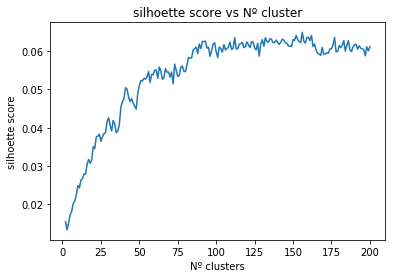
\includegraphics[scale=0.5]{KmeansSemPCASilhoette.png}
\\
\textbf{Figura 1}: \textit{Gráfico de k por Silhouette}
\end{center}

\begin{center}
\begin{tabular}{| l | l | l | l |}
 \hline
 \textbf{Clusters} &   \textbf{Score} &   \textbf{Calinski} &  \textbf{Silhoette} \\ \hline
2 &   -18038.0333456 &   312.302300127 &  0.0154703270706 \\ \hline
 20 &   -16451.1140207 &   119.058555969 &  0.0350597130577 \\ \hline
 40 &   -15527.5867898 &   91.7148367353 &  0.047632142909 \\ \hline
 60 &   -14899.7376406 &   77.3031750537 &  0.0550020513535 \\ \hline
 80 &   -14452.390996 &   67.2349438967 &  0.0546147507142 \\ \hline
 100 &   -14138.9536653 &   59.2252786152 &  0.0598284846652 \\ \hline
 120 &   -13838.2058328 &   53.9083198115 &  0.0623821272021 \\ \hline
 140 &   -13617.2681771 &   49.1624586366 &  0.0622077184482 \\ \hline
 160 &   -13467.8649372 &   44.7902655495 &  0.0636214443841 \\ \hline
 180 &   -13306.8956938 &   41.5605783281 &  0.0614516224447 \\ \hline
 200 &   -13183.9730324 &   38.6180843356 &  0.0611689653962 \\ \hline
\end{tabular} \newline

\textbf{Tabela 1}: \textit{Amostragem dos resultados do K-Means sem PCA}
\end{center}

\subsubsection{Análise dos medoids}
Medoide é um objeto que representa o cluster, é escolhido o objeto mais próximo do centroide como o medoide daquele cluster. Aqui vemos alguns medoids para avaliar a qualidade da clusterização.

\subsubsection{Com 80 clusters}
Selecionamos alguns medoids do modelo com \textit{k} = 80 para analise, e pegamos o assunto principal do texto:

\begin{itemize}

\item Cluster 1:
\begin{itemize}
\item Email 8518: venda de um pré-amplificador;
\item Email 8545: doutrina de Deus.
\end{itemize}

\item Cluster 2:
\begin{itemize}
\item Email 300: Baseball e sobre o melhor jogador da liga;
\item Email 14728: Empresa agrícola privada "DINA".
\end{itemize}

\item Cluster 3:
\begin{itemize}
\item Email 442: Compra de um sintetizador;
\item Email 1581: Natureza.
\end{itemize}

\item Cluster 4:
\begin{itemize}
\item Email 15899: Grampo do governo e criptografia;
\item Email 18219: Entrevista para ESPN em que Stanky diz que é polones, e não judeu.
\end{itemize}

\item Cluster 5:
\begin{itemize}
\item Email 17142: Um lance injusto em uma partida de hockey no gelo;
\item Email 2009: Problemas com MacBook.
\end{itemize}

\end{itemize}

\subsubsection{Com 47 clusters}

\begin{itemize}

\item Cluster 1:
\begin{itemize}
\item Email 11724: Lista de perguntas e respostas para uma ferramenta do Windows;
\item Email 18438: Coleções de objetos, como armas e vasos.
\end{itemize}

\item Cluster 2:
\begin{itemize}
\item Email 9778: Dúvida com o uso do compilador GCC;
\item Email 17347: Astronomia.
\end{itemize}

\item Cluster 3:
\begin{itemize}
\item Email 285: "Charlanismo" em alguns tratamentos médicos alternativos;
\item Email 1502: Foguetes.
\end{itemize}

\end{itemize}

\subsubsection{Conclusão da análise dos Medoids}
Pela análise superficial dos medoids, os clusters contem textos muito pouco relacionados.

\subsection{K-Means com PCA}
Foram testados diversos valores para a redução de variância de dados (0.85, 0.90, 0.93, 0.95 e 0.97). Apesar do pré-processamento e da redução de dimensionalidade, não foram observadas vantagens, tanto no custo computacional quanto no resultado do modelo. Dentre estes, o modelo que teve melhor desempenho foi o modelo com redução de 0.85. Possivelmente isso é explicado por que ao, reduzimos a dimensionalidade, nós também diminuimos a distância euclidiana dos membros dos cluster, o que resulta em uma Silhouette mais consistente com o restante e um score mais próximo a 1. Nesse modelo, com PCA de 0.85, o número de cluster mais adequado foi 100. Seu \textit{score} foi de -11398.3292007, \textit{Calinski} de 73.4076255749 e \textit{Silhoette} de 0.0704448614472.
 
\begin{center}
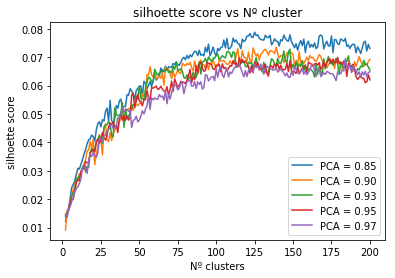
\includegraphics[scale=0.5]{KmeansSilhuetaComPCAs.png}
\\
\textbf{Figura 2}: \textit{Gráfico de k por Silhouette com PCA}
\end{center}
 
Para uma visualização gráfica aproximada da clusterização, reduzimos os dados para duas dimensões e obtivemos o seguinte gráfico de Voronoi \textit{k} = 80:
 
\begin{center}
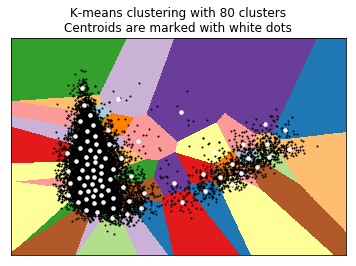
\includegraphics[scale=0.5]{80Clusters2D.png}
\\
\textbf{Figura 3}: \textit{Gráfico de Voronoi para a clusterização com 2 dimensões}
\end{center} 
 
Apesar da grande redução de dimensionalidade, é possível observar uma tendência para o posicionamento dos dados em uma região específica, onde os cluster podem ter tido dificuldade em lidar com as intersecções das classes. 

\subsection{K-Means nas bases geradas}
Utilizando conjunto de dados criados usados as \textit{stopwords} e os \textit{steamers} definidos na seção III, os emails originais foram pré-processados e criadas novas \textit{bag-of-words}. Os modelos tinham alto custo computacional para serem gerados e processados e, para testes, rodamos com dois \textit{k}s: 47 e 80. Esses números foram escolhidos após os resultados das seções anteriores. Todos as palavras foram convertidas para minúscula e as pontuações removidas. As palavras eram inseridas no \textit{bag-of-words} se elas aparecessem em mais de 2 textos e em menos de 800, para obtermos dados mais representativos. Os resultados com diferentes stemmers foram muito próximos, sugerindo que todos tem desempenho muito similar. Apesar da baixa amostragem de apenas dois valores de \textit{k}, os resultados tiveram métricas muito próximas e piores do que as encontradas nos testes anteriores, fazendo com que estes testes fossem descontinuados.\\


\begin{center}
\begin{tabular}{| l | l | l |}
 \hline
 \textbf{Clusters} &  \textbf{Stemmer}  &   \textbf{Score}  \\ \hline
47 &   WordNet &   -18594.0481 \\ \hline
47 &   Lancaster &   -18567.6497 \\ \hline
47 &   Snowball &  -18562.8424  \\ \hline
47 &   Porter &  -18571.6947  \\ \hline
80 &   WordNet &  -18372.5459  \\ \hline
80 &   Lancaster &  -18336.7877  \\ \hline
80 &   Snowball &  -18332.9902  \\ \hline
80 &   Porter &  -18332.8160  \\ \hline
\end{tabular} \newline

\textbf{Tabela 2}: \textit{Resultados obtidos com as bases geradas}
\end{center}

Contudo, uma vantagem deste modelo é conseguir verificar as palavras mais recorrentes de cada cluster, o que pode ser usado para verificar como o modelo está clusterizando os dados. Analisando, por exemplo, alguns clusters do modelo com WordNet e 47 clusters na tabela 3. \\
O cluster 4 se trata de assuntos ligados a esportes, o 31 também, porém com outros termos (incluindo baseball) enquanto o 46 parece se restringir ao baseball. Um email falando de baseball poderia permanecer na intersecção do 31 e 46, enquanto ele deveria de fato pertencer a ambos. Esse posicionamento nas margens dos clusters podem piorar o score do modelo.\\
Os clusters 1, 10 e 26 compartilham conceitos muito parecidos, caindo no mesmo problema de intersecção de assuntos. Embora os clusters consigam definir bem do que trata os assuntos dos seus componentes, o modelo aparenta falhar com assuntos que são muitos próximos, como, neste exemplo, cristianismo e religião.

\begin{center}
\begin{tabular}{| l | l | l |}
 \hline
 \textbf{Cluster} &  \textbf{Palavras mais populares}   \\ \hline
   4 & hockey win fan goal playoff cup espn \\ \hline
  31 & player baseball hockey nhl league players \\ \hline
  46 & pitcher hit win ball pitching hitter \\ \hline
   1 & church bible faith christ catholic jesus \\ \hline
  10 & atheist religion atheism belief faith exist \\ \hline
  26 & jesus christ georgia covington heaven \\ \hline
\end{tabular} \newline

\textbf{Tabela 3}: \textit{Palavras mais populares de alguns clusters do modelo com Wordnet e 47 cluster.}
\end{center}

\section{Conclusão}
Os resultados dos modelos de clusterização não obtiveram \textit{scores} razoáveis, levando a crer que o problema não seja ideal para o aprendizado não supervisionado. Conforme pode ser visto em \cite{b4}, a divisão original era composta de 20 grupos, porém com intersecção entre os grupos, onde um mesmo email pode pertencer a mais de um dos grupos. Os emails que ficam nessas intersecções acabam por gerar um \textit{score} ruim para o modelo, quando na verdade o ideal seria que o email pertence-se a mais de um dos clusters. A intersecção de clusters não é suportada pelo K-Means.\\
Acreditamos que a quantidade mais adequada de cluster é por volta de 90 para o algoritmo do K-Means, devido a sua aparente estabilização. A performance dos modelos em geral foi muito similar e nenhum deles é útil na prática.\\

\section{Estudos futuros}
Para conseguir resultados mais promissores, estudos futuros podem abordar outros pré-processamentos de textos e modelos supervisionados de classificação, já que a base de dados disponibiliza rótulos e classes sobres seus dados.

\begin{thebibliography}{00}

\bibitem{b1}Guzella, T. S., \& Caminhas, W. M. (2009). A review of machine learning approaches to spam filtering. Expert Systems with Applications, 36(7), 10206-10222.

\bibitem{b2}\texttt{\url{https://gmail.googleblog.com/2011/03/new-in-gmail-labs-smart-labels.html}}

\bibitem{b3}Tan, P. N. (2006). Introduction to data mining. Pearson Education India.

\bibitem{b4}\texttt{\url{http://qwone.com/~jason/20Newsgroups/}}

\bibitem{b5} Scikit-learn: Machine Learning in Python, acessado em 31 de Agosto de 2017, em \texttt{http://scikit-learn.org/stable/index.html}

\bibitem{b6} \texttt{\url{http://snowballstem.org/}}

\bibitem{b7} \texttt{\url{http://wordnet.princeton.edu/}}

\bibitem{b8} \texttt{\url{https://tartarus.org/martin/PorterStemmer/}}

\bibitem{b9} \texttt{\url{http://www.scientificpsychic.com/paice/paice.html}}

\bibitem{b10} \texttt{\url{https://ongspxm.github.io/blog/2014/12/bag-of-words-natural-language-processing/}}

\bibitem{b11} \texttt{\url{http://scikit-learn.org/stable/modules/generated/sklearn.cluster.KMeans.html}}

\bibitem{b12} \texttt{\url{http://scikit-learn.org/stable/modules/clustering.html\#calinski-harabaz-index}}

\bibitem{b13} \texttt{\url{www.facom.ufu.br/~backes/pgc204/Aula09-Agrupamentos.pdf}}

\bibitem{b14} \texttt{\url{http://www.nltk.org/}}

\end{thebibliography}

\end{document}
